\documentclass[12pt, a4paper, oneside]{ctexart}
\usepackage{amsmath, amsthm, amssymb, bm, color, framed, graphicx, hyperref, mathrsfs,enumerate,colortbl}
\title{\textbf{第三次作业}}
\author{1907402030 熊雄}
\date{\today}
\linespread{1.15}
\definecolor{shadecolor}{RGB}{241, 241, 255}
\newcounter{problemname}
\newenvironment{problem}{\begin{shaded}\stepcounter{problemname}\par\noindent\textbf{题目\arabic{problemname}. }}{\end{shaded}\par}
\newenvironment{solution}{\par\noindent\textbf{解答. }}{\par}
\newenvironment{note}{\par\noindent\textbf{题目\arabic{problemname}的注记. }}{\par}
\def\hth{\hat\theta}
\def\mA{\mathcal{A}}
\def\vv{1.2}
\usepackage{indentfirst}
\usepackage{booktabs}

 \begin{document}
 	\maketitle
\begin{problem}
	\textbf{(P50 d2.8)}
 	验证三种检验的关系
 	\begin{enumerate}
 		\item {\tt}
 		$ t = \frac{\hat{\beta_1}\sqrt{L_{xx}}}{\hat{\sigma}} = \frac{ \sqrt{n-2}r }{ \sqrt{1 - r^2 }} $
 		\item {\tt}
 		$ F = \frac{SSR / 1}{SSE / (n - 2)} =  \frac{\hat{\beta_1}^2 L_{xx}}{\hat{\sigma}^2}=  t^2 $

 	\end{enumerate}
\end{problem}



\begin{solution}
	
   	\begin{enumerate}
   	\item {\tt}    {\bf 证明:} 
   	  \begin{equation*}
     	\begin{split}
   	    t &=  \frac{\hat{\beta_1}\sqrt{L_{xx}}}{\hat{\sigma}}\\
    	&= \frac{\frac{L_{xy}}{L_{xx}}\sqrt{L_{xx}}}{\sqrt{\frac{1}{n-2}} \sqrt{\sum_{i=1}^{n}\left(y_i-\hat{y}\right)^2}}\\
    	&= \sqrt{n-2}r\frac{1}{\sqrt{\frac{\sum_{i=1}^n\left(y_i-\hat{y_i}\right)^2} {\sum_{i=1}^n\left(y_i-\bar{y_i}\right)^2}}}\\
    	&= \sqrt{n-2}r\frac{1}{\sqrt{\frac{\sum_{i=1}^n\left(y_i-\bar{y_i}\right)^2-\sum_{i=1}^n\left(\hat{y_i}-\bar{y_i}\right)^2} {\sum_{i=1}^n\left(y_i-\bar{y_i}\right)^2}}}\\
   	    &= \sqrt{n-2}r\frac{1}{\sqrt{1-\frac{\sum_{i=1}^n\left(\hat{y_i}-\bar{y_i}\right)^2}{\sum_{i=1}^n\left(y_i-\bar{y_i}\right)^2}}}\\
   	    &= \frac{\sqrt{n-2}r}{1-r^2}.
   	    \end{split}
   	  \end{equation*}
   	
   	\item {\tt }   {\bf 证明:}

   	  \[F =  \frac{SSR / 1}{SSE / (n - 2)}
   	  = \frac{r^2SST}{\sigma^2} 	  
   	 = \frac{(r)^2L_{yy}}{\sigma^2} 	 
   	  = \frac{\left(\frac{L_{xy}}{L_{xx}}\right)^2L_{xx}}{\sigma^2} 	 	 
   	  = \frac{\hat{\beta_1}^2 L_{xx}}{\hat{\sigma}^2}
   	  =  t^2. \]
   \end{enumerate} 
\end{solution}

\begin{problem}
	\textbf{(P50 d2.11)}
	验证决定系数$ r^2 $与$F$值之间的关系式\[ r^2 = \frac{F}{F+n-2}, \]
	以上表达式说明$ r^2 $与$F$值是等价的,那么我们为什么要分别引入这两个统计量,而不是只使用其中的一个?
\end{problem}

\begin{solution}
		\begin{enumerate}
		\item {\tt} 
	先验证关系式:
	\begin{equation*}
	\begin{split}
	r^2 &= \frac{SSR}{SST} \\
	&=  \frac{SSR}{SSR+SSE} \\
	&= \frac{1}{1+\frac{SSE}{SSR}} \\
	&= \frac{1}{1+\frac{n - 2}{F}} \\\
	&= \frac{F}{F+n-2}.
	\end{split}
	\end{equation*}
		\item {\tt} 引入这两个统计量的原因是这两个统计量研究的对象和目的都不同:
		\begin{enumerate}
			\item {\tt} 决定系数$r^2$是一个反映回归直线与样本观测值拟合优度的相对指标,如果决定系数$r^2$接近1,说明因变量不确定性的绝大部分能由回归方程解释,回归方程拟合优度好;反之,如果$r^2$不大,说明回归方程的效果不好,应进行修改,可以考虑增加新的自变量或者使用曲线回归。$r^2$的数值在0和1之间;
			\item{\tt}统计量$F$是对线性回归方程显著性的一种检验,其研究的是引起总平方和$SST$的两个因素$SSR$和$SSE$所占比重的多少,也就是如果回归平方和$SSR$越大回归的效果越好,回归方程便更显著。$F$的数值大于1.
			\end{enumerate}
	\end{enumerate}
\end{solution}
  
\begin{problem}
	\textbf{(P51 d2.14)}
	为了调查某广告对销售收入的影响,某商店记录了5个月的销售收入$ y $(万元)和广告费用$ x $(万元),数据如表1所示。请回答下面的问题:
	\begin{enumerate}
	\item{\tt 画散点图;}
    \item{\tt $x$与$y$之间是否大致呈线性关系?}
    \item{\tt 用最小二乘估计求出回归方程;}
    \item{\tt 求回归标准误差$\hat{\sigma}$;}
    \item{\tt 给出$\beta_0$与$\beta_1$的置信度为$95\%$的区间估计;}
    \item{\tt 计算$x$与$y$的决定系数;}
    \item{\tt 对回归方程做方差分析;}
    \item{\tt 做回归系数$\beta_1$的显著性检验;}	
    \item{\tt 做相关系数的显著性检验;}
    \item{\tt 对回归方程作残差图并做相应的分析;}
    \item{\tt 求当广告费用为$4.2$万元时,销售收入将达到多少,并给出置信度为$95\%$的置信区间。}
		\end{enumerate}
\end{problem}
\begin{table}[!htbp]
\begin{shaded} 
	\centering
	\caption{销售收入$ y $(万元)和广告费用$ x $(万元)}\label{tab:aStrangeTable}%添加标题 设置标签
	\begin{tabular}{cccccc}	
		\toprule
		月份& 1& 2& 3& 4& 5 \\
		\midrule
		$x$& 1& 2& 3& 4& 5\\
		\cline{1-6}  %为第1列到第6列添加横线
		$y$& 10& 10& 20& 20& 40\\
		\bottomrule
	\end{tabular}
	%\caption{这是一张三线表}\label{tab:aStrangeTable}  标题放在这里也是可以的
	\end{shaded}
\end{table}
 \begin{solution}
 	
 	\begin{enumerate}
 		\item {\tt}    {\bf 绘制散点图如下:} 
 		\begin{figure}[!h]	
 			\centering	
  			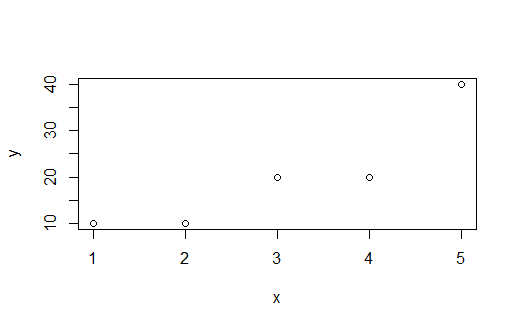
\includegraphics[scale=0.8]{plot1.png}
 			\label{图1}
 		\end{figure}  
 	   
        \item {\tt}    {\bf 答:}  
        由散点图可以看出$x$与$y$之间大致呈线性关系。
       
        \item {\tt}    {\bf 解:} 
        由表1可以计算得到:\[ \bar{x} = 3 ,\bar{y} = 20 ,L_{xy} = 70,  L_{xx} =10\]
        从而\[ \hat{\beta_1}=\frac{L_{xy}}{L_{xx}}= 7\]
        \[ \hat{\beta_0}=\bar{y} - \hat{\beta_1}\bar{x} = -1\]
        因此, 用最小二乘估计求出的回归方程为:
        \[  \hat{y} = -1 + 7 x .\]
        
        \item {\tt}    {\bf 解:} 
        计算得到回归标准误差:\[ \hat{\sigma}^2 = \frac{1}{n-2}\sum_{i=1}^n \left[y_i - (\hat{\beta_0} +\hat{\beta_1}x_i )^2 \right]= \frac{110}{3} \approx 36.67. \]
        
        
        \item {\tt}    {\bf 解:}
          \begin{enumerate}
    
          	  \item {\tt} 由于$\hat{\beta_1}\sim N(\beta_1,\frac{\hat{\sigma}^2}{L_{xx}})$, 故构造枢轴量\[ t = \frac{\left(\hat{\beta_1}-\beta_1\right)\sqrt{L_{xx}}}{\hat{\sigma}} \sim t(n-2).\]
          	 因此\[  P\left(\left| \frac{\left( \hat{\beta_1} - \beta_1 \right) \sqrt{L_{xx}}}{\hat{\sigma}} \right|<t_{\alpha/2}(n-2)\right)=1-\alpha.\]
          	 从而可以得到$\beta_1$的置信度为$1-\alpha$的置信区间为:
          	 \[ \left( \hat{\beta_1}-t_{\frac{\alpha}{2}}(n-2)\frac{\hat{\sigma}}{L_{xx}}, \hat{\beta_1}+t_{\frac{\alpha}{2}}(n-2)\frac{\hat{\sigma}}{L_{xx}}  \right). \]
          	 本题中我们令 $\alpha = 0.05$, 查表得$t_{0.025}(3)=3.1824$,从而计算得到$\beta_1$的置信度为$95\%$的置信区间为:
          	 \[ U_1=(5.0729,8.9271). \]
          
          	\item {\tt} 由于$\hat{\beta_0}\sim N\left(\beta_0,\left( \frac{1}{n}+ \frac{\left(\bar x\right)^2}{L_{xx}} \right)\sigma^2\right)$
          	, 故构造枢轴量\[ t = \frac{\hat{\beta_0}-\beta_0}{ \sqrt{\left( \frac{1}{n}+ \frac{\left(\bar x\right)^2}{L_{xx}} \right)\sigma^2}} \sim t(n-2).\]
          	因此\[  P\left(\left| \frac{\hat{\beta_0}-\beta_0}{ \sqrt{\left( \frac{1}{n}+ \frac{\left(\bar x\right)^2}{L_{xx}} \right)\sigma^2}} \right|<t_{\alpha/2}(n-2)\right)=1-\alpha.\]
          	从而可以得到$\beta_0$的置信度为$1-\alpha$的置信区间为:
          	\[ \left( \hat{\beta_0}-t_{\frac{\alpha}{2}}(n-2)\sqrt{\left( \frac{1}{n}+ \frac{\left(\bar x\right)^2}{L_{xx}} \right)\sigma^2}, \hat{\beta_0}+t_{\frac{\alpha}{2}}(n-2)\sqrt{\left( \frac{1}{n}+ \frac{\left(\bar x\right)^2}{L_{xx}} \right)\sigma^2}  \right). \]
          	本题中我们令 $\alpha = 0.05$, 查表得$t_{0.025}(3)=3.1824$,从而计算得到$\beta_0$的置信度为$95\%$的置信区间为:
          	\[U_2 = (-21.2119,19.2119). \]
        \end{enumerate}
        
        \item {\tt}    {\bf 解:} 
               $x$与$y$的决定系数为:
               \[ r^2 = \frac{L_{xy}^2}{L_{xx}L_{yy}} = \frac{49}{60} \approx 0.82.\]
               
        \item {\tt}    {\bf 解:} 
        原假设:\[ H_0 : \beta_1 = 0 \]
        对立假设: \[ H_1 : \beta_1 \neq 0 \]
        构造$F$检验统计量如下:\[ F=\frac{SSR / 1}{SSE / 3}, \]在正态假设下,当原假设$H_0$成立时,$F \sim F(1,3)$。查表得:$F_{1-0.05}(1,3)=10.13$ ,故拒绝域为:$ W_1 = \{ F>10.13\} . $
        计算得到:
        \[ SSR = \frac{l_{xy}^2}{l_{xx}}=490, SSE = l_{yy} - SSR = 110 ,\]
        从而
        \[ F =  \frac{147}{11} \approx 13.3636  >10.13.\]
        即在显著性水平$ \alpha = 0.05 $时,拒绝$ H_0 $ ,即回归效果是显著的。
        
        \item {\tt}    {\bf 解:} 
        原假设:\[ H_0 : \beta_1 = 0 \]
        对立假设: \[ H_1 : \beta_1 \neq 0 \]
        构造$t$检验统计量如下:\[ t = \frac{\left(\hat{\beta_1}-\beta_1\right)\sqrt{L_{xx}}}{\hat{\sigma}} . \]
        原假设$H_0$成立时, \[ t = \frac{\hat{\beta_1}L_{xx}}{\sigma^2}\sim t(n-2) \]
       
        \item {\tt}    {\bf 解:}
        原假设:\[ H_0 : r \neq 0 \]
        由\textbf{P50 d2.8}, 我们可以构造检验统计量\[ t = \frac{ \sqrt{n-2}r }{ \sqrt{1 - r^2 }} . \]
        在正态假设下,当原假设$H_0$成立时,$t \sim t_{\frac{\alpha}{2}}(n-2).$
        拒绝域为: \[W_2=  \{|t|> t_{\frac{\alpha}{2}}(n-2) \} .\] 
        计算得到\[ t = 3.6968 < 5.8409 = t_{0.005}(3).\]
        从而在显著性水平$ \alpha = 0.01 $时, 接受$ H_0 $, 即相关系数的效果是显著的。
        
        
        \item {\tt}    {\bf 解:}
         {\bf 绘制残差图如下:} 
        \begin{figure}[!h]	
        	\centering	
        	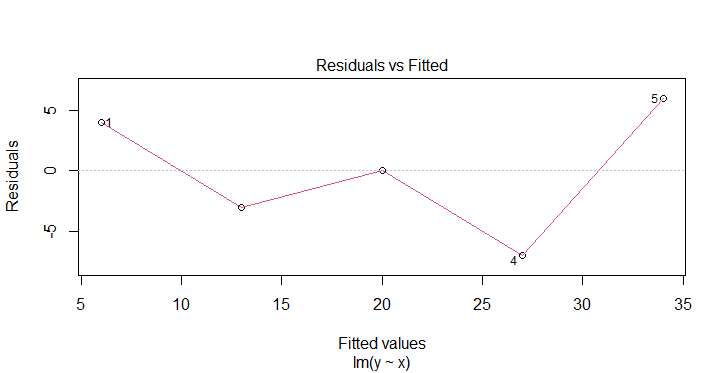
\includegraphics[scale=0.6]{plot2.png}
        	\label{图2}
        \end{figure}  
        
        
        从上图可以看出,残差的分布是比较均匀的,这样就代表误差分布模型的假设是满足的。
        
        
        \item {\tt}    {\bf 解:}
        在回归方程中,令$ x_0 = 4.2 $, 则$ y_0 = 28.4 $。即当广告费用为4.2万元时,销售收入将达到28.4万元。
        
        由于
        \[ \hat{y_0} \sim \left( \beta_0+\beta_1, \left(\frac{1}{n}+  \frac{\left(x_0 - \overline {x}\right)^2}{L_{xx}}\right)\hat{\sigma}^2 \right) ,\]
         记\[ h_{00} = \frac{1}{n}+  \frac{\left(x_0 - \overline {x}\right)^2}{L_{xx}}, \]
        则$ y_0 $的置信度为$ 1-\alpha $的置信区间为:
        \[ \left(\hat{y_0}-t_{\frac{\alpha}{2}}(n-2)\sqrt{1+h_{00}}\hat{\sigma}, ,\hat{y_0}+t_{\frac{\alpha}{2}}(n-2)\sqrt{1+h_{00}}\hat{\sigma} \right)\]
        通过计算可以得到$ y_0 $的置信度为$ 95\% $的置信区间为:\[ U_3 = (6.0586,50.7414). \]

    \begin{note}
    	本题的样本量很小,因此区间估计的误差较大。
    \end{note}

    \end{enumerate}
 \end{solution}
	
\end{document}

